% !TEX encoding = UTF-8 Unicode
% !TEX TS-program = xelatex
%%=================================================
%%
%% Department of Electrical and Computer Engineering
%% Project Report Template
%%
%% 1. "thesis.tex" - Only need to comment/uncomment parts that need compiled.
%%
%% 2. "info.tex" - Edit this file to define all your strings.
%%
%% 3. Edit these files for your report:
%%    1. abstract_th.tex       - บทคัดย่อ ภาษาไทย
%%    2. abstract_en.tex       - บทคัดย่อ ภาษาอังกฤษ
%%    3. ack_th.tex            - กิตติกรรมประกาศ ภาษาไทย
%%    4. ack_en.tex            - กิตติกรรมประกาศ ภาษาอังกฤษ (ไม่ได้ใช้)
%%    5. acronyms.tex          - คำย่อต่าง ๆ (ถ้ามี)
%%    6. chapter[1-5].tex      - รายงานแต่ละบท (บทที่ 1 - 5)
%%    7. refs.bib              - รายการเอกสารอ้างอิง
%%    8. appendix[A,B,...].tex - ภาคผนวก ก ข ...
%%
%%=================================================
\documentclass[12pt,a4paper,oneside]{book}
\newcommand{\mycomment}[1]{}

%%=================================================
%% START Packages
%%=================================================

%% Required packages for thesis layout (do not remove)
\usepackage{TUthesis}

%% Put everything else in "mystyle" package
\usepackage{mystyle}

%%=================================================
%% END Packages
%%=================================================


%%=================================================
%% START Project info
%%=================================================

%% Edit project information in the file "info.tex"
%%================================================
%% START Project info
%%================================================

%% Thesis for Master or Dissertation for PhD
\newcommand{\thesistype}{Thesis}

%% Thesis title in mixed case
\newcommand{\titleThai}{REST API สำหรับการส่งงานเขียนโปรแกรมด้วย OpenAPI 2}
\newcommand{\titleEng}{REST API for Programming Assignment with OpenAPI 2}

%% Student name(s) i.e. author(s) of this thesis
%% Order suggestion: by alphabetical order
\newcommand{\authorAThai}{นาย นภทีป์ ละปะชัย}
\newcommand{\authorBThai}{นาย ธาม พลศรีสุทธิกุล}
\newcommand{\authorAEng}{Mr. Napatee Lapachai}
\newcommand{\authorBEng}{Mr. Tharm Pholsrisuthikul}


%% Degree that this thesis is for
\newcommand{\degreeThai}{วิศวกรรมศาสตรบัณฑิต}
\newcommand{\degreeEng}{Bachelor of Engineering}

%% Major
\newcommand{\majorThai}{วิศวกรรมคอมพิวเตอร์}
\newcommand{\majorEng}{Computer Engineering}

%% Date of submission
\newcommand{\submissionDayThai}{26}
\newcommand{\submissionDayEng}{26}
\newcommand{\submissionMonthThai}{พฤษภาคม}
\newcommand{\submissionMonthEng}{May}
\newcommand{\submissionYearThai}{2566}
\newcommand{\submissionYearEng}{2023}

%% Academic year for thesis submission
\newcommand{\academicYearThai}{2565}
\newcommand{\academicYearEng}{2022}

%% Institute/department
\newcommand{\facultyThai}{คณะวิศวกรรมศาสตร์}
\newcommand{\facultyEng}{Faculty of Engineering}

%% keywords
\newcommand{\keywordThai}{REST API, OpenAPI, งานเขียนโปรแกรม}
\newcommand{\keywordEng}{REST API, OpenAPI, programming assignment}

\newcommand{\headOfDepartmentThai}{ผู้ช่วยศาสตราจารย์ ดร. พิศาล แก้วประภา}
\newcommand{\headOfDepartmentEng}{Asst. Dr. Phisan Kaewprapha}
\newcommand{\advisorThai}{อาจารย์ นาวิน สมญาติ}
\newcommand{\advisorEng}{Mr. Nawin Somyat}

\newcommand{\committeeA}{อาจารย์ ดร. พิศาล แก้วประภา }
\newcommand{\committeeB}{อาจารย์ นาวิน สมญาติ}
%\newcommand\dean{รองศาสตราจารย์ ดร. ธีร์ เจียศิริพงษ์กุล}

%%-----------------------------
%% No need to edit after this
%%-----------------------------

%% case author is empty
\newcommand{\authorAEngNew}{ \ifthenelse{\equal{\authorAEng}{}} {~} {\authorAEng} }
\newcommand{\authorAThaiNew}{ \ifthenelse{\equal{\authorAThai}{}} {~} {\authorAThai} }
\newcommand{\authorBEngNew}{ \ifthenelse{\equal{\authorBEng}{}} {~} {\authorBEng} }
\newcommand{\authorBThaiNew}{ \ifthenelse{\equal{\authorBThai}{}} {~} {\authorBThai} }
%%================================================
%% END Project info
%%================================================


%%=================================================
%% END Project info
%%=================================================

%%+++++++++++++++++++++++++++++++++++++++++++++++++
%% EDIT - Uncomment the type of report to compile
%%+++++++++++++++++++++++++++++++++++++++++++++++++
\setReportType{Sample}
%\setReportType{Proposal}
%\setReportType{Progress 1}
%\setReportType{Progress 2}
%\setReportType{Final}

%%+++++++++++++++++++++++++++++++++++++++++++++++++
%% EDIT - Uncomment this line if you have acronyms page
%%+++++++++++++++++++++++++++++++++++++++++++++++++
\addAcronyms{true}

%%+++++++++++++++++++++++++++++++++++++++++++++++++
%% EDIT - Uncomment this line if you have listings page
%%+++++++++++++++++++++++++++++++++++++++++++++++++
\addListOfListings{true}

%%+++++++++++++++++++++++++++++++++++++++++++++++++
%% EDIT - Uncomment this line if you have appendix page(s)
%%+++++++++++++++++++++++++++++++++++++++++++++++++
\addAppendix{true}


%%#################################################
%% No need to edit anything below this.
%%#################################################

\begin{document}
\frontmatter

\addtocontents{toc}{\contheading}
\setlength{\parskip}{0pt plus1pt minus1pt}

%%=================================================
%% First page - Thai with logo
%%=================================================

\pagestyle{empty}
\begin{center}
	\vspace*{6mm}
	\begin{center}
		%
\includegraphics[width=1in]{tu-logo-bw.jpg}\\
		
\includegraphics[width=1in]{tu-logo-color.jpg}\\
	\end{center}
	\vspace{1cm}

	\begin{spacing}{1.4}
		\textbf{\huge\titleThai}
	\end{spacing}
	\vspace*{35mm}
	\textbf{โดย}\\
	\vspace*{10mm}
	\textbf{\authorAThaiNew}\\
	\textbf{\authorBThaiNew}\\
	\vfill

	\begin{spacing}{1.3}
		\textbf{โครงงานนี้เป็นส่วนหนึ่งของการศึกษาตามหลักสูตร\\
			\degreeThai\\
			สาขา\majorThai\\
			\facultyThai\ มหาวิทยาลัยธรรมศาสตร์\\
			ปีการศึกษา \academicYearThai\\
			ลิขสิทธิ์ของมหาวิทยาลัยธรรมศาสตร์}
	\end{spacing}
\end{center}

%%=================================================
%% Second page - thai without logo
%%=================================================
\pagestyle{empty}
\begin{center}
	\vspace*{40mm}
	\begin{spacing}{1.4}
		\textbf{\huge\titleThai}
	\end{spacing}
	\vspace*{35mm}
	\textbf{โดย}\\
	\vspace*{10mm}
	\textbf{\authorAThaiNew}\\
	\textbf{\authorBThaiNew}\\
	\vfill
	\begin{spacing}{1.3}
		\textbf{โครงงานนี้เป็นส่วนหนึ่งของการศึกษาตามหลักสูตร\\
			\degreeThai \\ สาขา\majorThai\\
			\facultyThai ~ มหาวิทยาลัยธรรมศาสตร์  \\
			ปีการศึกษา \academicYearThai\\ ลิขสิทธิ์ของมหาวิทยาลัยธรรมศาสตร์}
	\end{spacing}
\end{center}

%%=================================================
%% Third page - English without logo
%%=================================================
\pagestyle{empty}
\begin{center}
	\vspace*{40mm}
	\begin{spacing}{1.4}
		\textbf{\huge\titleEng}
	\end{spacing}
	\vspace*{35mm}
	\textbf{BY}\\
	\vspace*{10mm}
	\textbf{\authorAEngNew}\\
	\textbf{\authorBEngNew}\\
	\vfill
	\begin{spacing}{1.3}
		\textbf{A PROJECT SUBMITTED IN PARTIAL FULFILLMENT OF THE\\
			REQUIREMENTS FOR THE DEGREE OF BACHELOR OF ENGINEERING\\
			IN COMPUTER ENGINEERING\\
			FACULTY OF ENGINEERING\\ THAMMASAT UNIVERSITY\\
			ACADEMIC YEAR \academicYearEng\\ COPYRIGHT OF THAMMASAT UNIVERSITY}
	\end{spacing}
\end{center}

%%=================================================
%% Signatures page
%%=================================================
\vspace*{2mm}
\begin{center}
	มหาวิทยาลัยธรรมศาสตร์\\
	\textnormal{\facultyThai} \\
	\vspace*{10mm}
	โครงงาน\\
	\vspace*{10mm}
	ของ\\
	\vspace*{10mm}
	\authorAThaiNew\\
	\authorAThaiNew\\
	\vspace*{10mm}
	เรื่อง\\
	\vspace*{10mm}
	\titleThai \\
	\vspace*{10mm}
	\begin{spacing}{1.3}
		ได้รับการตรวจสอบและอนุมัติ ให้เป็นส่วนหนึ่งของการศึกษาตามหลักสูตร\\
		\degreeThai
	\end{spacing}
	\vspace*{8mm}
	เมื่อวันที่ ~ \submissionDayThai ~ \submissionMonthThai ~ พ.ศ. \submissionYearThai \\
\end{center}
\vspace*{2mm}
%\vfill
%~Approved as to style and content by\\[-2ex]
\begin{table}[H]
	%\setlength{\tabcolsep}{2.7ex}
	\renewcommand{\arraystretch}{1.3}
	\begin{tabular}{c c c}
		อาจารย์ที่ปรึกษาโครงงาน                &  &                         \\ \cline{3-3}
		                                   &  & (\advisorThai)          \\[3ex]
		หัวหน้าภาควิชาวิศวกรรมไฟฟ้าและคอมพิวเตอร์ &  &                         \\ \cline{3-3}
		                                   &  & (\headOfDepartmentThai) \\[3ex]
	\end{tabular}
\end{table}


%%=================================================
%% Abstract page - Thai
%%=================================================
% do not edit here; instead edit the file abstractth.tex

\setlength{\parindent}{0.8in}
\pagestyle{plain}
\setcounter{page}{1}
\renewcommand{\thepage}{(\arabic{page})} %\setcounter{page}{-1}

\begin{table}[H]
	\setlength{\tabcolsep}{0.7ex}
	\begin{tabular}{l c l}
		หัวข้อโครงงาน           &  & \titleThai         \\
		ชื่อผู้เขียน               &  & \authorAThaiNew    \\
		                      &  & \authorBThaiNew    \\
		ชื่อปริญญา               &  & \degreeThai        \\
		สาขาวิชา/คณะ/มหาวิทยาลัย &  & \majorThai         \\
		                      &  & \facultyThai       \\
		                      &  & มหาวิทยาลัยธรรมศาสตร์ \\
		อาจารย์ที่ปรึกษาโครงงาน   &  & \advisorThai       \\
		ปีการศึกษา              &  & \academicYearThai  \\
	\end{tabular}
\end{table}

\addcontentsline{toc}{section}{บทคัดย่อ}
\addtocontents{toc}{\protect\vspace{\baselineskip}}

\begin{center} \textbf{\Large บทคัดย่อ} \end{center}
%%================================================
%% Abstract - Thai
%%================================================

โครงงาน REST API สําหรับการส่งงานเขียนโปรแกรมด้วย OpenAPI จัดทําขึ้นเพื่ออํานวยความสะดวกให้กับบุคคลากรทางการศึกษาเพื่อใช้ในการตรวจโจทย์ปัญหาประเภทเขียนโปรแกรม โดยโครงงานมีลักษณะเป็นการพัฒนา REST API จํานวน 2 ตัว เพื่อใช้ในการส่งงานประเภทเขียนโปรแกรม โดยแบ่งออกเป็น compile API สําหรับ compile โปรแกรม และ problem API เปรียบเทียบระหว่างไฟล์คำตอบและเฉลย \\
\indent โดย API ทั้งสองตัวจะมีรูปแบบการทํางานที่แตกต่างกัน กล่าวคือ compile API มีหน้าที่สําหรับให้ผู้ใช้งานส่ง request ซึ่งเป็นไฟล์งานและ input ที่ต้องการใส่เพื่อทำการเรียกใช้โปรแกรม (ใส่หรือไม่ใส่ก็ได้) และจากนั้น API จะทำการ compile ไฟล์นั้นและใส่ input ให้ (หากมี) หากไม่มีข้อผิดพลาดจะส่ง output ออกมาเป็น response ในขณะที่ problem API มีหน้าที่สําหรับเปรียบเทียบระหว่างไฟล์คำตอบและเฉลย โดยการตรวจสอบว่า input เดียวกัน output ที่ออกมาจะเป็นเหมือนกันหรือไม่ และส่งผลลัพธ์ออกมาเป็น response \\
\indent โครงงานนี้ได้มีการใช้ภาษา Go และพัฒนาด้วย Gin framework ซึ่งสร้างมาเพื่อพัฒนา REST API นอกจากนี้ยังมีการพัฒนา API บนแพลตฟอร์ม Docker เพื่อให้สามารถรองรับการใช้งานได้อย่างหลากหลายตามความต้องการของผู้ใช้




\vspace{8mm}
\noindent \textbf{คำสำคัญ:} \keywordThai


\newpage
%%=================================================
%% Abstract page - English
%%=================================================
% do not edit here; instead edit the file abstract.tex
\begin{table}[H]
	%\setlength{\tabcolsep}{0.7ex}
	\begin{tabular}{l c l}
		Title                          &  & \titleEng            \\
		Author                         &  & \authorAEngNew       \\
		                               &  & \authorBEngNew       \\
		Degree                         &  & \degreeEng           \\
		Major Field/Faculty/University &  & \majorEng            \\
		                               &  & \facultyEng          \\
		                               &  & Thammasat University \\
		Advisor                        &  & \advisorEng          \\
		Academic Year                  &  & \academicYearEng     \\
	\end{tabular}
\end{table}

\addcontentsline{toc}{section}{Abstract}
\addtocontents{toc}{\protect\vspace{\baselineskip}}

\begin{center} \textbf{\Large ABSTRACT} \end{center}
%%================================================
%% Abstract - English
%%================================================

This project is created to provide convenience to educational personnel for checking programming assignment. This project is split into two REST APIs which are compile API for compiling the program and problem API for comparing between answer and file to be checked. \\
\indent These two APIs have different operation. The compile API is responsible for the user who needs to compile a program by sending a request to compile API with source code and input (if any) then API will compile a program , send input to the program that been compiled and send output to be a response. On the other hand, the problem API is for comparing between two files by getting the same input then compare between output of each file after that the result will be a response of the API. \\
\indent This project uses Go as main computer language and is developed with Gin framework and can be deployed using Docker platform so it can be used in many opportunities.


\vspace{8mm}
\noindent \textbf{keyword:} \keywordEng

%%=================================================
%% Acknowledgement page - Thai
%%=================================================
% do not edit here; instead edit the file ackth.tex
\chapter*{กิตติกรรมประกาศ \\[-1em]}
%%================================================
%% Acknowledgements - Thai
%%================================================

ขอขอบคุณ

\addcontentsline{toc}{section}{กิตติกรรมประกาศ}
\addtocontents{toc}{\protect\vspace{\baselineskip}}

%%=================================================
%% Table of Contents, Figures and Tables
%%=================================================
% comment/uncomment any tables/lists that you desire
\cleardoublepage
\phantomsection
\addcontentsline{toc}{section}{สารบัญ}
\addtocontents{toc}{\protect\vspace{\baselineskip}}
\tableofcontents

%\newpage
%%=================================================
%% Figures page
%%=================================================
\cleardoublepage
\phantomsection
\addcontentsline{toc}{section}{สารบัญรูป}
\addtocontents{toc}{\protect\vspace{\baselineskip}}
\listoffigures

%\newpage
%%=================================================
%% Tables page
%%=================================================
\cleardoublepage
\phantomsection
\addcontentsline{toc}{section}{สารบัญตาราง}
\addtocontents{toc}{\protect\vspace{\baselineskip}}
\listoftables


%\newpage
%%=================================================
%% Listings page
%%=================================================


\IfAddAcronyms{
	%%=================================================
%% Acronym page
%%=================================================
% do not edit here; instead edit the file acronyms.tex
\cleardoublepage
\phantomsection
\addcontentsline{toc}{section}{สัญลักษณ์และคำย่อ}
\addtocontents{toc}{\protect\vspace{\baselineskip}}
\chapter*{สัญลักษณ์และคำย่อ \\[-1em]}
%%================================================
%% Acronyms/Abbreviations
%%================================================
\begin{tabular}{ll}
    \textbf{สัญลักษณ์/คำย่อ} & \textbf{คำเต็ม/คำจำกัดความ}                            \\\\
    IKE                  & Internet Key Exchange                                \\[1.5ex]
    SSH                  & Secure Shell                                         \\[1.5ex]
    PIN                  & Personal Identification Number                       \\[1.5ex]
    ePIN                 & Electronic Personal Identification Number            \\[1.5ex]
    SMS                  & Short Message Service                                \\[1.5ex]
    ID                   & Identifier                                           \\[1.5ex]
    HTTPS                & Hypertext Transfer Protocol over Secure Socket Layer \\[1.5ex]
    FIDO                 & Fast IDentity Online                                 \\[1.5ex]
    UAF                  & Universal Authentication Framework                   \\[1.5ex]
    ASM                  & Authenticator Specific Module
\end{tabular}

}
%%=================================================
%% Chapters
%%=================================================
\mainmatter

%% Edit the files chapter1.tex, chapter2.tex, ...

%% บทนำ
%% Introduction
%%================================================
%% Chapter 1
%%================================================
\chapter{บทนำ}
%\label{intro}
\label{chapter1}

\section{ที่มาและความสำคัญ}
    ข้อดีและข้อเสียของอินเทอร์เน็ต มีมากมาย เช่น เพื่อการทําธุรกรรมทางการเงิน ส่งผล\mbox{ให้}การซื้อขายง่ายขึ้น แต่มีความเสี่ยงในการถูกหลอกหลวงได้ง่ายด้วยเช่นกัน การใช้งานอินเทอร์เน็ตเพื่อการศึกษาก็มีข้อเสีย เช่น การที่ผู้สอนขาดปฏิสัมพันธ์กับผู้เรียนโดยตรง หรือการที่ถูกสิ่งเร้าจากภายนอกคอย\mbox{รบกวน} จากสาเหตุข้างต้น จึงเป็นที่มาของโครงงาน REST API สําหรับการส่งงานเขียนโปรแกรมด้วย OpenAPI (REST API for Programming assignment With OpenAPI) ที่จะยกระดับการทําการบ้านหรือการทําข้อสอบประเภทการเขียนโปรแกรมในรูปแบบออนไลน์ ให้มีความปลอดภัยมากขึ้น และสามารถตรวจสอบความถูกต้องได้ รวมถึงเป็นการอํานวยความสะดวกให้แก่อาจารย์หรือผู้สอนในการตรวจข้อสอบ ป้องกันไม่ให้เกิดการตรวจข้อสอบที่ผิดพลาด และสามารถลดเวลาในการตรวจข้อสอบได้เป็นอย่างมาก

\section{วัตถุประสงค์}
\begin{enumerate}
    \item เพื่อพัฒนา API ตามแนวทางของ REST API สําหรับการส่งงานเขียนโปรแกรม
    \item เพื่อพัฒนาระบบสําหรับรองรับการเรียกใช้ API ในการการส่งงานเขียนโปรแกรม
    \item เพื่อเพิ่มความรวดเร็วในการส่งงานหรือส่งข้อสอบการเขียนโปรแกรม
    \item เพื่ออํานวยความสะดวกให้ผู้สอนสําหรับการตรวจงานการเขียนโปรแกรม
    \item เพื่อเพิ่มความแม่นยําและถูกต้องในการตรวจงานการเขียนโปรแกรม
\end{enumerate}


\section{ขอบเขตการดำเนินงาน}
\begin{enumerate}
    \item พัฒนา API ตามแนวทางของ REST API สําหรับการส่งงานเขียนโปรแกรม โดยจะพัฒนา API 2 รายการดังนี้
    \begin{enumerate}[\theenumi.\arabic*]
        \item API รายการแรกเป็น Compile API ทําหน้าที่ตรวจสอบโปรแกรม และส่งผลลัพธ์ของโปรแกรมกลับมาเป็น output
        \item API รายการที่สองเป็น Problem API  ทําหน้าที่รับข้อมูลจากผู้ใช้และทําการตรวจสอบโปรแกรม โดยทําการเปรียบเทียบกับผลเฉลย และส่งผลลัพธ์กลับเป็น output
    \end{enumerate}        
    \item API ที่พัฒนาทั้ง 2 รายการ จะรับข้อมูลคําตอบได้เฉพาะไฟล์ที่เป็นภาษาคอมพิวเตอร์
\end{enumerate}
\section{ขั้นตอนการดำเนินงาน}
\begin{enumerate}
    \item เริ่มศึกษาค้นคว้าเกี่ยวกับเรื่องที่ผู้จัดทำต้องใช้ในโครงงาน
    \item กำหนดขอบเขตที่จะทำหลังจากสรุปแนวทางที่ได้จากอาจารย์ที่ปรึกษา
    \item พูดคุยกับผู้ร่วมโครงงานเกี่ยวกับการแบ่งหน้าที่ และ จัดแบ่งภาระงานอย่างเหมาะสม
    \item ลงมือทำโครงงานตามที่ได้รับมอบหมาย
    \item ทดสอบการใช้งานของ API
    \item จัดทำรายงาน
    \item นำเสนอโครงงาน
\end{enumerate}

\section{ผลที่คาดว่าจะได้รับ}
ผู้จัดทำโครงงานคาดหวังว่า ผู้ใช้จะได้รับประโยชน์การใช้ service เพื่อแบ่งเบาภาระ\mbox{หน้าที่}ในการตรวจข้อสอบ ลดเวลาในส่วนการตรวจซึ่งไม่จำเป็น และสำหรับผู้ที่เป็นนักศึกษาจะสามารถมีช่องทางการส่งข้อสอบได้อย่างสะดวก และทราบผลได้อย่างรวดเร็วยิ่งขึ้น
\begin{landscape}

\section{ตารางการดำเนินงาน}

    \begin{table}[h]
        \centering
        
        \begin{tabular}{|*{21}{c|}}
        \hline 
        \multirow {2}{*}{หัวข้อ} & \multicolumn{4}{c|}{สิงหาคม} & \multicolumn{4}{c|}{กันยายน} & \multicolumn{4}{c|}{ตุลาคม} & \multicolumn{4}{c|}{พฤศจิกายน} & \multicolumn{4}{c|}{ธันวาคม} \\\cline {2-21}
        & 1 & 2 & 3 & 4 & 1 & 2 & 3 & 4 &  1 & 2 & 3 & 4 & 1 & 2 & 3 & 4 & 1 & 2 & 3 & 4  \\\hline 
         สรุปแนวทางการจัดทำภายในคณะผู้จัดทำ & x & x &  &  &  &  &  &  &  &  &  &  &    &  &  &  &  &  &  &  \\\hline 
         จัดทำรายงานข้อเสนอโครงงาน &  &  & x &  &  &  &  &  &  &  &  &  &  &  &  &  &  &  &  &    \\\hline 
         นำส่งรายงาน และปรับแก้รายงานกับอาจารย์ที่ปรึกษา &  &  &  & x  &  &  &  &  &  &  &  &  &  &  &  &  &  &  &  &  \\\hline 
         จัดทำรายงานการค้นคว้าเบื้องต้น &  &  &  &  & x & x  & x  & x  &  &  &  &  &  &  &  &  &  &  &  & \\\hline 
        จัดทำโครงงานในส่วนอื่น ๆ &  &  &  &  &  &  &  &  & x & x & x & x &  &  &  &  &  &  &  &   \\\hline 
        จัดทำรายงานความคืบหน้าและสอบครั้งที่ 1 &  &  &  &  &  &  &  &  &  &  &  &  & x & x & x & x &  &  &  &   \\\hline 
         อัปเดตความคืบหน้า &  &  &  &  &  &  &  &  &  &  &  &  &  &  &  &  & x & x & x & x  \\\hline 
        
        \end{tabular}
        \caption{การดำเนินโครงงาน}
        \label{tab:my_label}
        \vspace{0.5em}
    
        \begin{tabular}{|*{21}{c|}}
        \hline 
         \multirow {2}{*}{หัวข้อ} & \multicolumn{4}{c|}{มกราคม} & \multicolumn{4}{c|}{กุมภาพันธ์} & \multicolumn{4}{c|}{มีนาคม} & \multicolumn{4}{c|}{เมษายน} & \multicolumn{4}{c|}{พฤษภาคม} \\\cline {2-21}
        & 1 & 2 & 3 & 4 & 1 & 2 & 3 & 4 &  1 & 2 & 3 & 4 & 1 & 2 & 3 & 4 & 1 & 2 & 3 & 4  \\\hline 
         อัปเดตความคืบหน้า จัดทำรายงานความคืบหน้าโครงงานครั้งที่ 2  & x & x & x & x & x & x &  &  &  &  &  &  &    &  &  &  &  &  &  &  \\\hline 
         ทดสอบการใช้งานของ  &  &  &  &  &  &  & x & x &  &  &  &  &  &  &  &  &  &  &  &    \\\hline 
         จัดทำโครงงานให้แล้วเสร็จ  &  &  &  &  &  &  &  &  & x & x & x & x &  &  &  &  &  &  &  &  \\\hline 
         ตรวจสอบความเรียบร้อยและจัดทำปริญญานิพนธ์และบทความ &  &  &  &  &  &   &   &   &  &  &  &  & x & x & x & x &  &  &  & \\\hline 
        สอบโครงงานครั้งที่ 2 และส่งปริญญานิพนธ์ฉบับสมบูรณ์ &  &  &  &  &  &  &  &  &  &  &  &  &  &  &  &  & x &  &  &   \\\hline 
    
        \end{tabular}
        \caption{การดำเนินโครงงาน (ต่อ)}
        \label{tab:my_label}
    \end{table}


    



\end{landscape}


%% ทฤษฎีหรืองานที่เกี่ยวข้อง
%% Literature Review
%%================================================
%% Chapter 2
%%================================================
\chapter{ทฤษฎีหรืองานที่เกี่ยวข้อง}
%\label{literature}
\label{chapter2}

\section{หัวข้อใหญ่}

\subsection{หัวข้อย่อยระดับที่ 1}

\subsubsection{หัวข้อย่อยระดับที่ 2}

\section{หัวข้อใหญ่}

\subsection{หัวข้อย่อยระดับที่ 1}

\subsubsection{หัวข้อย่อยระดับที่ 2}


%% การดําเนินงาน
%% Methodology
%%================================================
%% Chapter 3
%%================================================
\chapter{การดําเนินงาน/วิธีวิจัย}
%\label{method}
\label{chapter3}

\section{ศึกษาการเขียนภาษา Go}
    ภาษาที่ใช้เขียน API นั้นมีหลากหลายภาษาไม่ว่าจะเป็น Python, Java, Kotlin หรือ Dart เป็นต้น โดยผู้จัดทำเลือกใช้ภาษา Go เนื่องจากขนาดและประเภทของงานตรงตามจุดประสงค์ที่สุดคือ การพัฒนา REST API และมี framework ที่เหมาะสมกับงานที่สุดนั่นคือ Gin framework ที่สร้างขึ้นมาเพื่อพัฒนา REST API โดยเฉพาะ

\subsection{หัวข้อที่เกี่ยวกับภาษา Go}

\subsubsection{ภาษา Go}
    ได้ทำการศึกษาการเขียน ภาษา Go\cite{Go} เพื่อนำมาสร้าง API เนื่องจากเป็นภาษาที่ได้รับความนิยมมากขึ้นเรื่อย ๆ ในยุคนี้โดยภาษา Go นั้นจะมีจุดเด่นในเรื่องของ Performance ที่\mbox{ทำงาน}ได้อย่างรวดเร็วเทียบกับภาษาอื่น ๆ อีกทั้งยังมีจุดเด่นคือความง่ายในการเขียนและการอ่าน และยัง\mbox{สามารถ}ทำ Concurrent Programming ได้ง่าย เพราะภาษา Go ถูกออกแบบมาเพื่อทำให้ Application ที่ต้องใช้ Multi-Threading หรือ Distributed Systems เป็นเรื่องที่ง่ายขึ้น
\subsubsection{Gin framework}
    หลังจากที่ได้ศึกษาหลากหลาย framework แล้ว ผู้จัดทำได้เลือกเป็น Gin framework\cite{Gin} เนื่องจาก Gin framework เป็น framework ที่ถูกสร้างขึ้นมาเพื่อ REST API และ มี feature หรือ libraries ที่สําคัญเหมาะกับ service ที่มีขนาดเล็กไม่มีความซับซ้อนมาก มีการแบ่งกลุ่ม API เพื่อความสะดวกในการใช้งาน
    
\section{ออกแบบ REST API ด้วยมาตรฐาน OAS}
OAS หรือ OpenAPI Specification เป็นมาตรฐานในการอธิบาย REST API ตัวหนึ่ง ๆ ที่สร้างมาเพื่อให้มนุษย์และคอมพิวเตอร์สามารถอ่านได้ โดยหลังจากเขียน OAS เสร็จสิ้น จะสามารถใช้เป็นแบบแผน เพื่อช่วยในการสร้าง พัฒนา และปรับปรุง REST API ให้ตรงกับ OAS ที่ได้ออกแบบไว้เพื่อการทํางานที่เป็นระบบและมีเป้าหมายที่ชัดเจน

\subsection{รูปแบบของ OpenAPI Specification}
        \begin{figure}[H]
            \centering
                \centering
                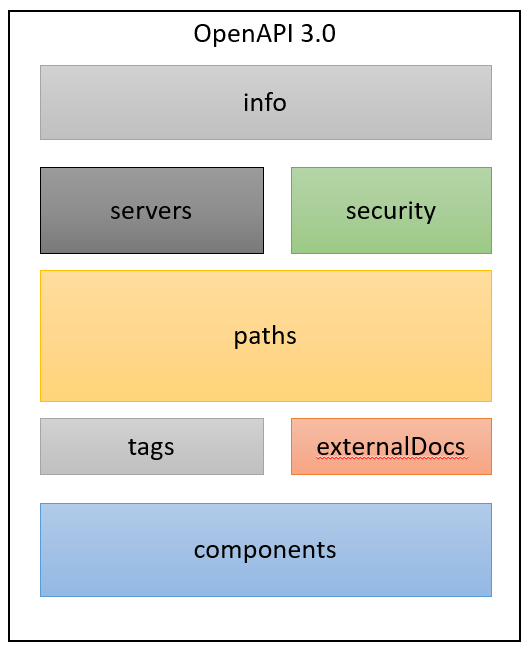
\includegraphics[width=5in]{latex/figures/openapi3.png}
            \captionsource{โครงสร้างของ OpenAPI}{\url{https://swagger.io/blog/api-design/openapi-driven-api-design/}}
        \end{figure}
จากโครงสร้าง OpenAPI ดังในรูปที่ 3.1 มีรายละเอียดดังนี้

\subsubsection{OpenAPI}
\raggedright ส่วนนี้จะเป็นการแสดงเวอร์ชันของ OpenAPI ที่ใช้ในการเขียน Specification ชุดนั้น ๆ
\subsubsection{Info}
\raggedright ส่วนนี้จะเป็นส่วนที่แสดงข้อมูลทั่วไปของ REST API คือ ชื่อ API, รายละเอียดเบื้องต้น, \mbox{ใบอนุญาติ} (license) ที่ใช้, ช่องทางการติดต่อ (contact) ของเจ้าของ API หรือ Terms of Service
\subsubsection{Servers}
\raggedright ส่วนนี้จะแสดงข้อมูลเกี่ยวกับเซิร์ฟเวอร์ที่ตั้งของ API
\subsubsection{Paths}
\raggedright ส่วนนี้เป็นส่วนที่ใหญ่ที่สุดใน Specification โดยเป็นส่วนที่แสดง Endpoint หรือ Path ต่าง ๆ ของ
API รวมถึง Operation ที่สามารถใช้กับ Endpoint นั้นได้ โดยในที่นี้ก็คือ HTTP verb ต่าง ๆ เช่น Get,
Post, Put, Delete เป็นต้น โดยในแต่ละ Path จะมีรายละเอียดดังนี้
     \begin{enumerate}
    \item รายชื่อกลุ่มที่มี Operation สามารถมีได้หลาย tag ใน Path เดียวกัน
    \item summary - ระบุความหมายและหน้าที่ของ Operation
    \item description - ระบุรายละเอียดการทํางานของ Operation
    \item operationId - เป็นค่า identity ของ Operation มักตั้งชื่อตรงกับชื่อฟังก์ชันในโค้ด เพื่อความสะดวกและป้องกันความสับสนเมื่ออ่านโค้ด
    \item security - ลักษณะของ Authentication ที่ต้องใช้ใน Operation นั้น
    \item requestBody - เป็นรายละเอียดของข้อมูลที่ต้องส่งมาให้ Operation ผ่านทาง RequestBody มักใช้ใน Operation ประเภท POST, PUT
    \item  parameters - สําหรับกําหนดรายละเอียดของข้อมูลที่ต้องส่งมาให้ Operation ทาง Query, Path, Header
    \item responses - สําหรับกําหนดรายละเอียดของข้อมูลที่ Operation จะทําการส่งกลับมาเมื่อทํางานเสร็จสิ้นแล้ว
\end{enumerate}

\subsubsection{Tags}
\raggedright ส่วนนี้เป็นส่วนไว้รวบรวมชื่อที่ใช้จัดกลุ่มของ Operation เพื่อให้สะดวกในการอ่านค่า response
\subsubsection{ExternalDocs}
\raggedright ส่วนนี้เป็นส่วนที่แสดง URL ของเว็บไซต์ที่มีข้อมูลนอกเหนือจาก Specification
\subsubsection{Components}
\raggedright ส่วนที่รวบรวมโครงสร้างต่าง ๆ เพื่อให้สามารถนําเฉพาะส่วน header ไปใช้ในส่วนอื่น ๆ ใน Specification
ได้ผ่านฟังก์ชัน reference

\subsection{การออกแบบ API ด้วยมาตรฐาน OpenAPI Specification}
หลังจากวางแผนรูปแบบของ REST API ที่ต้องการจะสร้างเสร็จสิ้นแล้ว ได้เริ่มทําการออกแบบ
OpenAPI Specification ผ่าน OpenAPI Editor Tool ที่มีชื่อว่า Stoplight Studio
\subsubsection{Stoplight Workspace}
    กําหนด Path จํานวน 2 Path คือ Path compile และ Path problem เพื่อเป็น
ตัวแทน API ทั้ง 2 ตัว หลังจากนั้นได้ทําการกําหนดรายละเอียดต่าง ๆ ภายใน Path ดังกล่าว ได้ออก
มาเป็นมาตรฐาน OpenAPI Specification โดยให้อยู่ในรูปของ YAML file format
        \begin{figure}[H]
            \centering
                \centering
                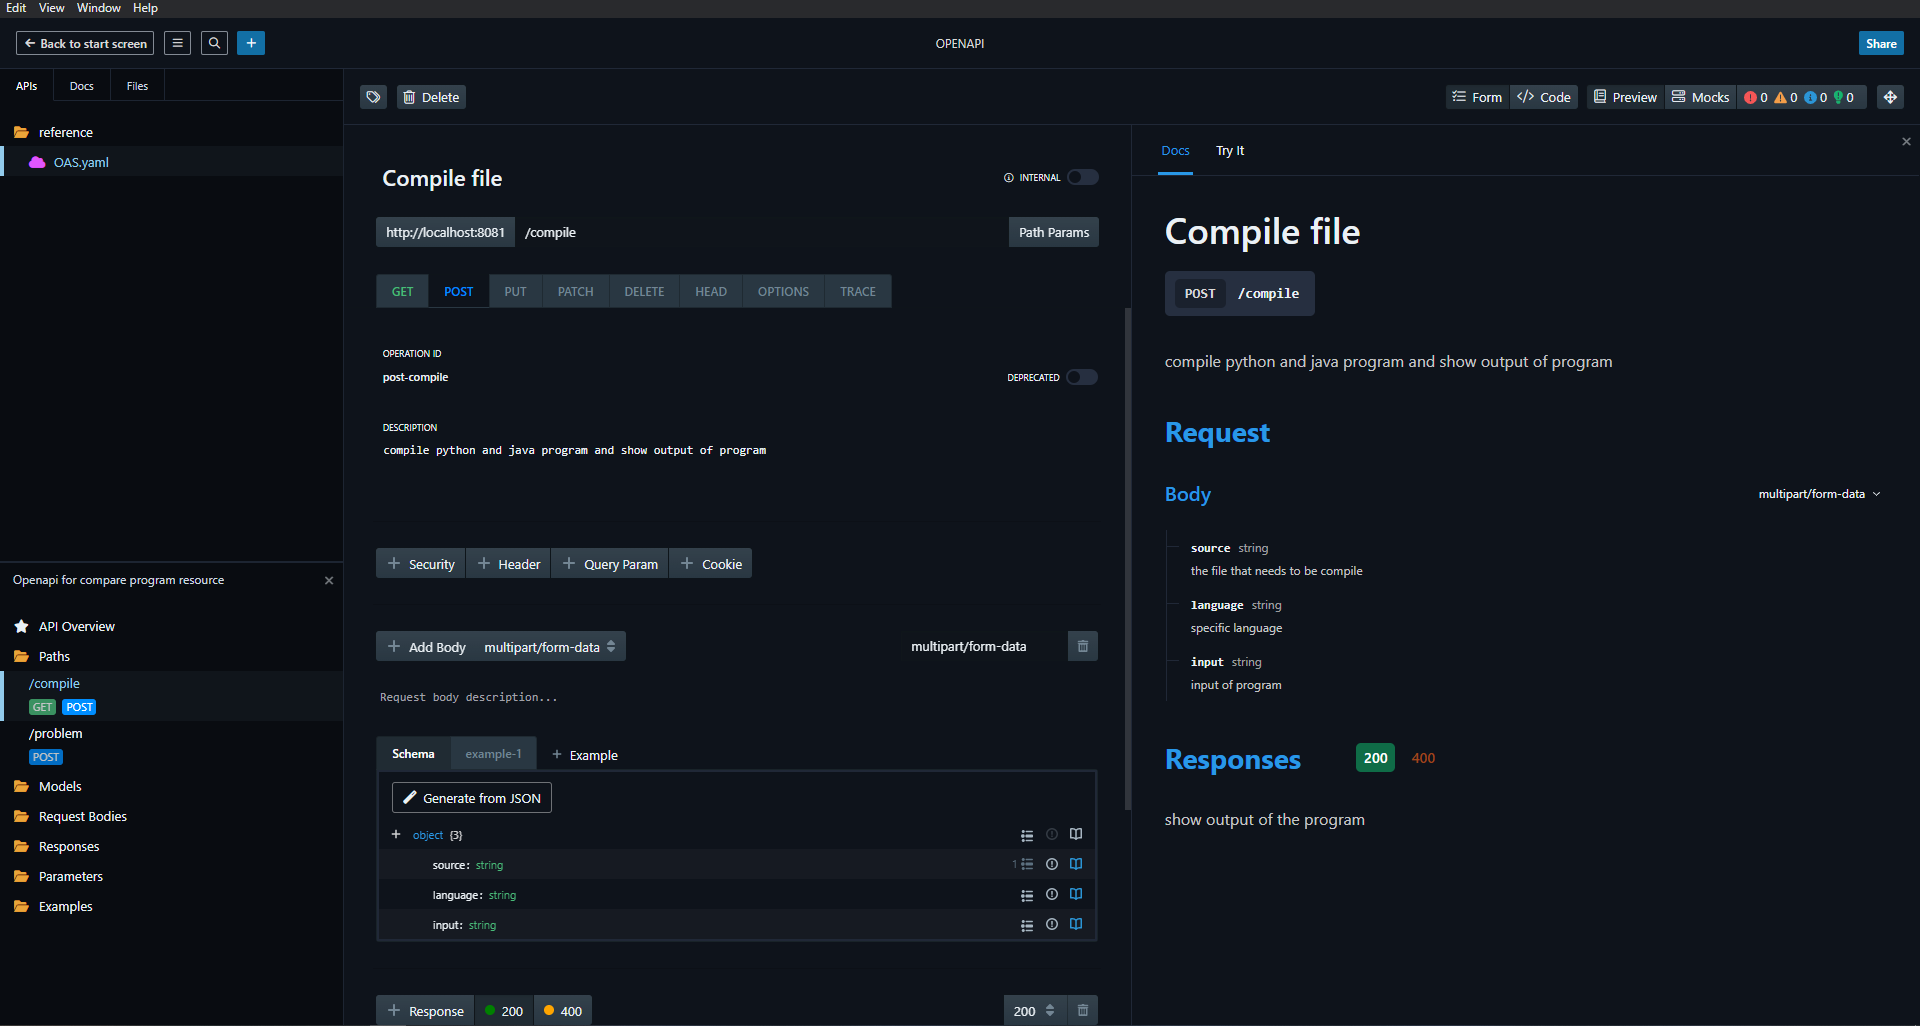
\includegraphics[width=5in]{latex/figures/stoplight.png}
            \caption{Stoplight Editor}
        \end{figure}
        \begin{figure}[H]
            \centering
                \centering
                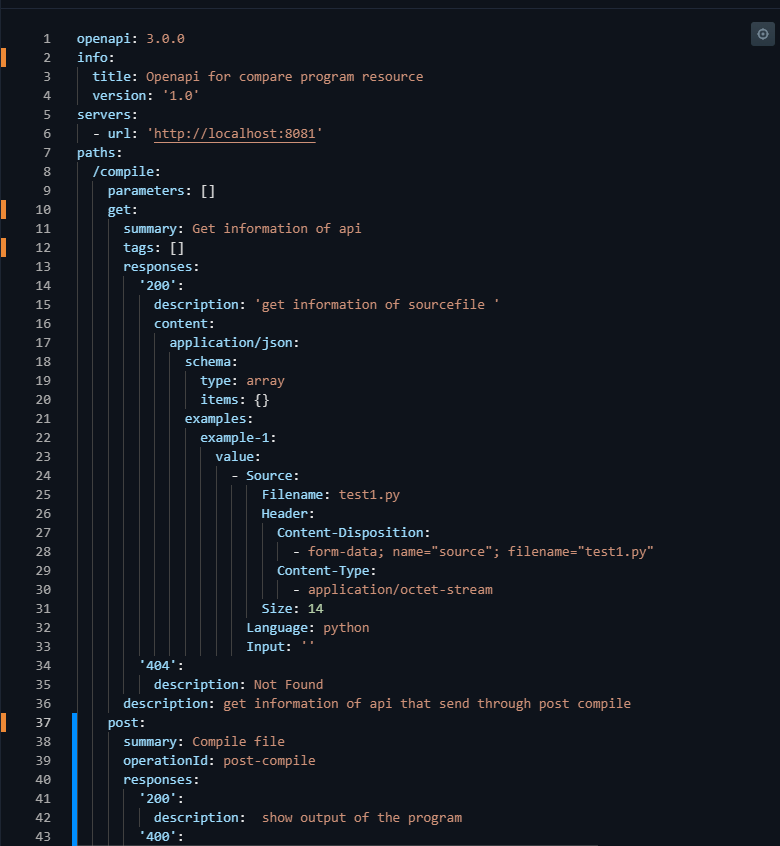
\includegraphics[width=5in]{latex/figures/OAS.png}
            \caption{OpenAPI Specification}
        \end{figure}

\section{การสร้างเอกสารประกอบ (API Documentation)}
หลังจากได้ออกแบบ API ตาม OAS เป็นไฟล์ในรูปแบบ YAML แล้ว จะเป็นการสร้างเอกสาร
ประกอบ หรือการสร้าง API Document กล่าวคือ เป็นเอกสารที่ช่วยให้การสื่อสารระหว่าง ส่วนการทํางาน
แบบด้านหน้า (Front-end) และด้านหลัง (Back-end) สามารถสื่อสารกันได้สะดวกมากยิ่งขึ้น โดยได้
เลือกใช้ OpenAPI Document Tool ที่มีชื่อว่า APITree ในการสร้างเอกสารประกอบดังกล่าว

        \begin{figure}[H]
            \centering
                \centering
                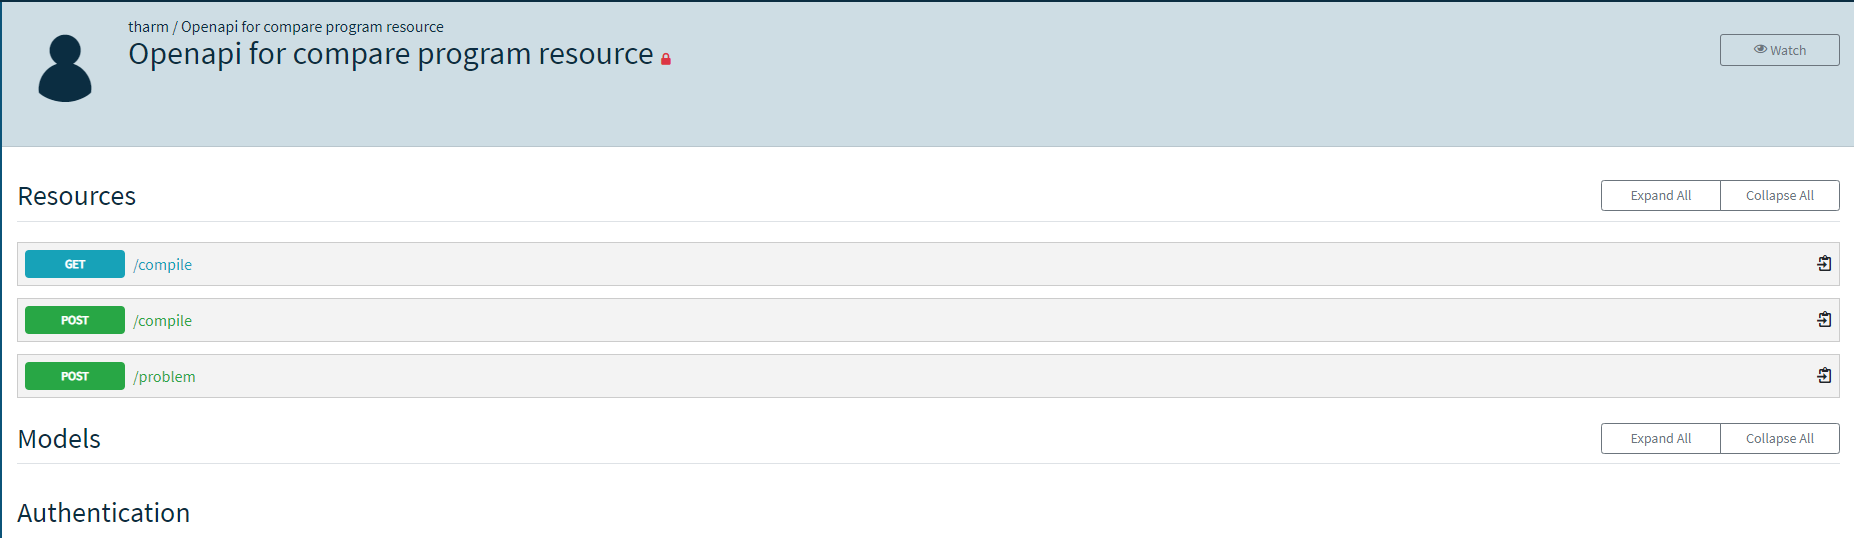
\includegraphics[width=5in]{latex/figures/apitree.png}
            \captionsource{APITree Document Page}{\url{https://hub.apitree.com/tharm/Openapi/}}
        \end{figure}
        \begin{figure}[H]
            \centering
                \centering
                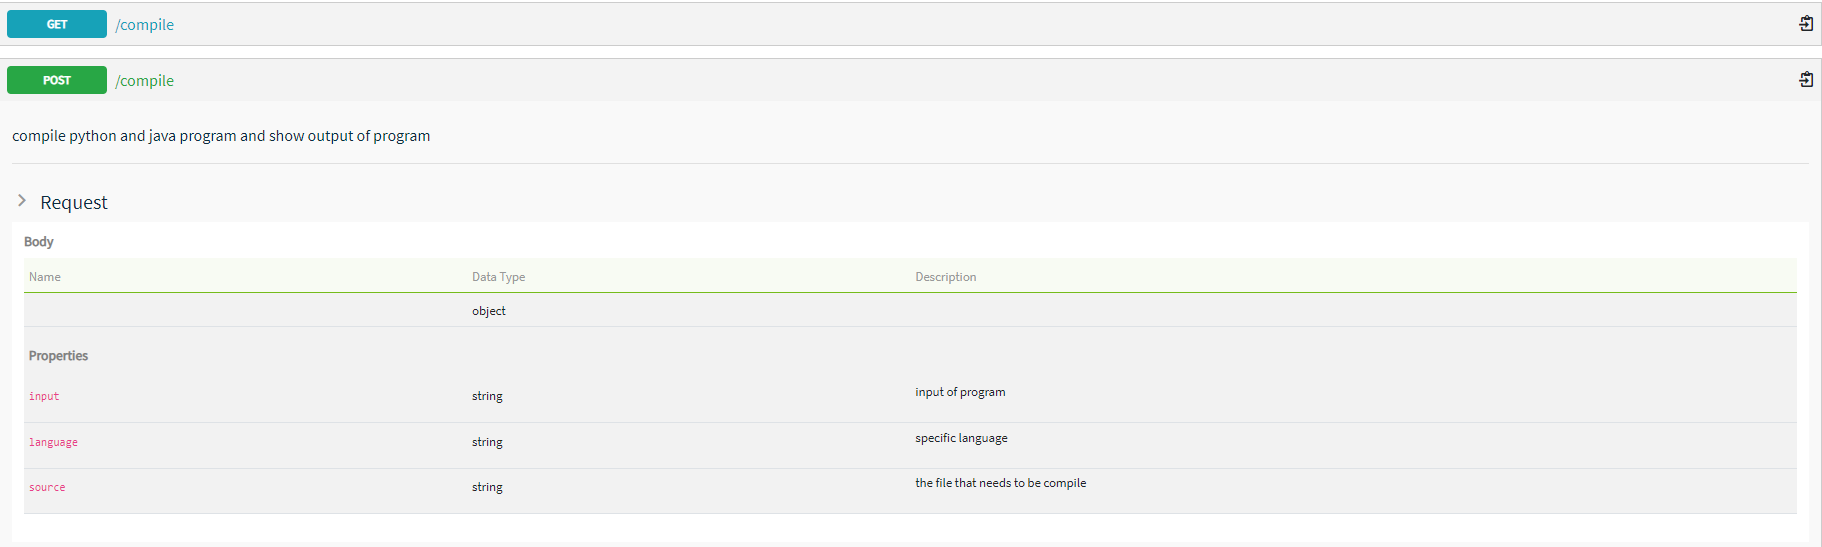
\includegraphics[width=5in]{latex/figures/apitree_detail.png}
            \captionsource{APITree Document Detail}{\url{https://hub.apitree.com/tharm/Openapi/}}
        \end{figure}
\section{การใช้งาน Docker Engine}
ในช่วงหลังของการพัฒนา ได้มีการนํา Docker \cite{docker} มาปรับใช้กับระบบการพัฒนา
ส่วนเบื้องหลัง โดยมีการสร้าง Docker image ขึ้นมาจากการเขียน Dockerfile และไฟล์ docker compose
\cite{compose} เพื่อให้ระบบ API สามารถทํางานได้บนคอมพิวเตอร์ทุกเครื่องที่ต้องการ และมีความสะดวกและ
รวดเร็ว ซึ่งเป็นคุณสมบัติเด่นของ Docker engine



%% ผลการดำเนินงาน
%% Finding and Results
%%================================================
%% Chapter 4
%%================================================
\chapter{ผลการดำเนินงานและอภิปรายผล}
%\label{result}
\label{chapter4}

\section{หัวข้อใหญ่}

\subsection{หัวข้อย่อยระดับที่ 1}

\subsubsection{หัวข้อย่อยระดับที่ 2}

\section{หัวข้อใหญ่}

\subsection{หัวข้อย่อยระดับที่ 1}

\subsubsection{หัวข้อย่อยระดับที่ 2}



%% สรุปโครงงาน
%% Conclusions and Recommendations
%%================================================
%% Chapter 5
%%================================================
\chapter{สรุปผลการดำเนินงาน อุปสรรค และการพัฒนาในอนาคต}
%\label{conclusion}
\label{chapter5}

\section{สรุปผลโครงงาน}

\subsection{หัวข้อย่อยระดับที่ 1}

\section{ปัญหาและอุปสรรค}

\subsection{หัวข้อย่อยระดับที่ 1}

\section{ข้อเสนอแนะในการพัฒนาต่อ}

\subsection{หัวข้อย่อยระดับที่ 1}


%% ตัวอย่างการเขียน
%% Examples of writing LaTeX
\chapter{ตัวอย่างการเขียน LaTeX}
\label{example}

\section{โครงสร้างของ Template}
ในไฟล์ zip ประกอบด้วยไฟล์ต่าง ๆ ดังต่อไปนี้
\begin{enumerate}[1.]
    \item \filename{thesis.tex} เป็นไฟล์หลักที่ประกอบด้วย ไฟล์ย่อยต่างๆ ตลอดจนข้อมูลของวิทยานิพนธ์ เช่น ชื่อวิทยานิพนธ์ทั้งภาษาไทย และอังกฤษ ชื่อผู้แต่ง ชื่อกรรมการสอบวิทยานิพนธ์
    \item \filename{info.tex} - ไฟล์ที่กำหนดข้อมูลของโครงงาน
    \item \filename{abstract_th.tex} - ไฟล์ที่เขียนบทคัดย่อ ภาษาไทย
    \item \filename{abstract_en.tex} - ไฟล์ที่เขียนบทคัดย่อ ภาษาอังกฤษ
    \item \filename{acronyms.tex} - ไฟล์ที่เขียนสัญลักษณ์ หรือคำย่อ (ถ้าใช้)
    \item \filename{ack_th.tex} - ไฟล์ที่เขียนกิตติกรรมประกาศ ภาษาไทย
    \item \filename{ack_en.tex} - ไฟล์เขียนกิตติกรรมประกาศ ภาษาอังกฤษ (ไม่ใช้ไฟล์นี้)
    \item \filename{chapter[1..5].tex} - ไฟล์ของบทต่าง ๆ ศึกษารายละเอียดของบทต่าง ๆ ในคู่มือวิทยานิพนธ์~\cite{tu:2556fk}
    \item \filename{appendix[A..B].tex} - ไฟล์ภาคผนวก %% โดยภาคผนวกมีได้สูงสุด 10 ภาคผนวก
    \item \filename{refs.bib} - ไฟล์ฐานข้อมูลรายการอ้างอิง (Bibliography) ในรูปแบบ BibTeX
    \item \filename{TUthesis.sty} - ไฟล์ template style สำหรับมหาวิทยาลัยธรรมศาสตร์ (ไม่จำเป็นต้องแก้ไขไฟล์นี้)
    \item \filename{mystyle.sty} - ไฟล์ template style สำหรับปรับแต่งรายงานโครงงาน (ไม่จำเป็นต้องแก้ไขไฟล์นี้)
    \item \filename{example.tex} - ไฟล์ตัวอย่างการเขียน LaTeX
\end{enumerate}

\newpage
\section{การเขียน LaTeX}
สามารถอ่านจากบทความต่าง ๆ
\begin{enumerate}[1.]
    \item บทแนะนำ LaTeX 2e แบบไม่ค่อยย่อ แปลโดย คุณจักรภาษณ์ วิศวกุล\\
    \url{http://zelmanov.ptep-online.com/ctan/lshort_thai.pdf}

    %%\item ตัวอย่างคำสั่ง LaTeX ของภาควิชาคณิตศาสตร์ คณะวิทยาศาสตร์ ม. เชียงใหม่\\
    %% Link down
    %%\url{http://www.math.science.cmu.ac.th/thanasak/pow/CMU_LaTeX_2010_All.pdf} %%
    \item บทแนะนำ LaTeX 2e แบบไม่ค่อยย่อ ภาษาอังกฤษ โดย Tobias Oetiker\\
    \url{https://tobi.oetiker.ch/lshort/lshort.pdf}

    \item ตัวอย่างคำสั่ง LaTeX ของภาควิชาคณิตศาสตร์ คณะวิทยาศาสตร์ ม. เกษตรศาสตร์\\
    \url{http://maths.sci.ku.ac.th/th/service/training/2556/2555-06-17_1/doc_xelatex.pdf}

    \item Thesis template และแนะนำการใช้ LaTeX ของอาจารย์ \mbox{ดร. ฑิตยา หวานวารี}  ภาควิชาคณิตศาสตร์และวิทยาการคอมพิวเตอร์ คณะวิทยาศาสตร์ จุฬาลงกรณ์มหาวิทยาลัย\\
    \url{http://pioneer.netserv.chula.ac.th/~wdittaya/}

    \item LaTeX ใน Wikibook\\
    \url{https://en.wikibooks.org/wiki/LaTeX}

    \item การใช้ Endnote กับ Latex และ BibTeX\\
    \url{http://www.rhizobia.co.nz/latex/convert}
\end{enumerate}

\newpage
\section{การใช้ฟอนต์}
\
ฟอนต์หลักที่ได้กำหนดไว้แล้วในรายงานคือ \texttt{TH Sarabun New} การใช้งานฟอนต์ สามารถเลือกรูปแบบการแสดงได้ดังนี้

\begin{table}[H]
    \centering
    \footnotesize
    \begin{threeparttable}
        \caption{รูปแบบการแสดงฟอนต์}
        \label{tab:font style}
        \begin{tabular}{l c C{6cm} c}
            \toprule
            \textbf{รูปแบบ} & \textbf{คำสั่ง} & \textbf{ตัวอย่างการใช้คำสั่ง} & \textbf{ผลการแสดง} \\
            \midrule
            ตัวหนา & \verb|\textbf{text}| & \verb|\textbf{|พลังของแผ่นดิน\verb|}| & \textbf{พลังของแผ่นดิน} \\
            ตัวเอียง & \verb|\textit{text}| & \verb|\textit{|พลังของแผ่นดิน\verb|}| & \textit{พลังของแผ่นดิน} \\
            ตัวเอียงและหนา & \verb|\textit{\textbf{text}}| & \verb|\textit{\textbf{|พลังของแผ่นดิน\verb|}}| & \textit{\textbf{พลังของแผ่นดิน}} \\
            ตัวหนาและเอียง & \verb|\textbf{\textit{text}}| & \verb|\textbf{\textit{|พลังของแผ่นดิน\verb|}}| & \textbf{\textit{พลังของแผ่นดิน}} \\
            ขีดเส้นใต้ & \verb|\underline{text}| & \verb|\underline{|พลังของแผ่นดิน\verb|}| & \underline{พลังของแผ่นดิน} \\
            ตัวหนาและเอียง\footnotetext[1]{test} & \verb|\underline{\textit{text}}| & \verb|\underline{\textit{|พลังของแผ่นดิน\verb|}}| & \underline{\textit{พลังของแผ่นดิน}} \\
            เน้นข้อความ\tnote{1} & \verb|\emph{text}| & \verb|\emph{|พลังของแผ่นดิน\verb|}| & \emph{พลังของแผ่นดิน} \\
            \bottomrule
        \end{tabular}
        \begin{tablenotes}
            \item [1] ปกติจะแสดงเป็นแบบเดียวกับตัวเอียง (italic)
        \end{tablenotes}
    \end{threeparttable}
\end{table}

LaTeX มีคำสั่งในการเปลี่ยนขนาดฟอนต์ แต่สำหรับในรายงานโครงงาน ไม่จำเป็นต้องเปลี่ยนขนาดฟอนต์ คำสั่งใน \autoref{tab:font size} เหล่านี้จะเปลี่ยนขนาดของฟอนต์ที่ใช้ในสภาพแวดล้อม\mbox{ปัจจุบัน} จนกว่าจะมีการใช้คำสั่งเปลี่ยนขนาดใหม่

\begin{table}[H]
    \centering
    \footnotesize
    \begin{threeparttable}
        \caption{เปลี่ยนขนาดของฟอนต์}
        \label{tab:font size}
        \begin{tabular}{l C{6cm} c}
            \toprule
            \textbf{คำสั่ง} & \textbf{ตัวอย่างการใช้คำสั่ง} & \textbf{ผลการแสดง} \\
            \midrule
            \verb|\tiny| & \verb|\tiny| พลังของแผ่นดิน & \tiny พลังของแผ่นดิน \\
            \verb|\scriptsize| & \verb|\scriptsize|พลังของแผ่นดิน| & \scriptsize พลังของแผ่นดิน \\
            \verb|\footnotesize| & \verb|\footnotesize| พลังของแผ่นดิน & \footnotesize พลังของแผ่นดิน \\
            \verb|\small| & \verb|\small| พลังของแผ่นดิน & \small พลังของแผ่นดิน \\
            \verb|\normalsize| & \verb|\normalsize|พลังของแผ่นดิน & \normalsize พลังของแผ่นดิน \\
            \verb|\large| & \verb|\large| พลังของแผ่นดิน & \large พลังของแผ่นดิน \\
            \verb|\Large| & \verb|\Large| พลังของแผ่นดิน & \Large พลังของแผ่นดิน \\
            \verb|\LARGE| & \verb|\LARGE| พลังของแผ่นดิน & \LARGE พลังของแผ่นดิน \\
            \verb|\huge| & \verb|\huge| พลังของแผ่นดิน & \huge พลังของแผ่นดิน \\
            \verb|\Huge| & \verb|\Huge| พลังของแผ่นดิน & \Huge พลังของแผ่นดิน \\
            \bottomrule
        \end{tabular}
    \end{threeparttable}
\end{table}

ในกรณีที่ต้องการเปลี่ยนขนาดฟอนต์เฉพาะบางส่วนของข้อความ ให้เขียนคำสั่งภายในสภาพแวดล้อมปิด (อยู่ภายในเล็บวงเล็บปีกกา) เช่น \verb|{\footnotesize test}|

\newpage
\section{การเพิ่มรายการ (List)}

รูปแบบคำสั่งในการเขียนรายการใน LaTeX คือ

\begin{lstlisting}[caption={รูปแบบคำสั่งในการเขียนรายการ (list)}, label={list:list format},language=TeX]
\begin{|\textcolor{blue}{list\_type}|}
    \item รายการที่ 1
    \item รายการที่ 2
    \item รายการที่ 3
\end{|\textcolor{blue}{list\_type}|}
\end{lstlisting}

โดย \textcolor{blue}{\texttt{list\_type}} ใน \autoref{list:list format} มีอยู่ 3 แบบคือ

\begin{itemize}[noitemsep]
    \item \textbf{\color{blue}itemize} รายการแบบใช้สัญลักษณ์ (เช่น bullet point)
    \item \textbf{\color{blue}enumerate} รายการแบบใช้ตัวเลข (หรือตัวอักษร เช่น 1. (a))
    \item \textbf{\color{blue}description} รายการแบบการอธิบายคำ
\end{itemize}

%%=================================================
%% Itemize
%%=================================================

\subsection{ตัวอย่างรายการแบบ \textcolor{blue}{itemize}}

\begin{exampleBox}[sidebyside]{รายการแบบ defaut (bullet)}
\begin{lstlisting}[frame=none,language={[LaTeX]TeX}]
\begin{itemize}
    \item รายการที่ 1
    \item รายการที่ 2
    \item รายการที่ 3
\end{itemize}
\end{lstlisting}
\tcblower
\begin{itemize}[noitemsep]
    \item รายการที่ 1
    \item รายการที่ 2
    \item รายการที่ 3
\end{itemize}
\end{exampleBox}


\begin{exampleBox}[sidebyside]{รายการซ้อนกัน (nested list)}
\small
\begin{lstlisting}[frame=none,language={[LaTeX]TeX}]
\begin{itemize}
    \item รายการระดับ 1
    \begin{itemize}
        \item รายการระดับ 2
        \begin{itemize}
            \item รายการระดับ 3
            \begin{itemize}
                \item รายการระดับ 4
            \end{itemize}
        \end{itemize}
    \end{itemize}
\end{itemize}
\end{lstlisting}
\tcblower
\small
\begin{itemize}[noitemsep,leftmargin=*,label=\textbullet]
    \item รายการระดับ 1
    \begin{itemize}
        \item รายการระดับ 2
        \begin{itemize}
            \item รายการระดับ 3
            \begin{itemize}
                \item รายการระดับ 4
            \end{itemize}
        \end{itemize}
    \end{itemize}
\end{itemize}
\end{exampleBox}


\begin{exampleBox}[lefthand ratio=0.55,sidebyside]{เปลี่ยนสัญลักษณ์ที่ระดับต่าง ๆ}
\small
\begin{lstlisting}[frame=none,language={[LaTeX]TeX}]
\begin{itemize}[\textbullet]
    \item รายการระดับ 1
    \begin{itemize}[\textendash]
        \item รายการระดับ 2
        \begin{itemize}[$\ast$]
            \item รายการระดับ 3
            \begin{itemize}[$\square$]
                \item รายการระดับ 4
            \end{itemize}
        \end{itemize}
    \end{itemize}
\end{itemize}
\end{lstlisting}
\tcblower
\small
\begin{itemize}[\textbullet,noitemsep,leftmargin=*,]
    \item รายการระดับ 1
    \begin{itemize}[\textendash]
        \item รายการระดับ 2
        \begin{itemize}[$\ast$]
            \item รายการระดับ 3
            \begin{itemize}[$\square$]
                \item รายการระดับ 4
            \end{itemize}
        \end{itemize}
    \end{itemize}
\end{itemize}
\end{exampleBox}

%%=================================================
%% Enumerate
%%=================================================

\subsection{ตัวอย่างรายการแบบ \textcolor{blue}{enumerate}}

\begin{exampleBox}[sidebyside]{รายการมีลำดับแบบ defaut (ลำดับเป็นตัวเลขอารบิก)}
\begin{lstlisting}[frame=none,language={[LaTeX]TeX}]
\begin{enumerate}
    \item รายการที่ 1
    \item รายการที่ 2
    \item รายการที่ 3
\end{enumerate}
\end{lstlisting}
\tcblower
\begin{enumerate}[noitemsep]
    \item รายการที่ 1
    \item รายการที่ 2
    \item รายการที่ 3
\end{enumerate}
\end{exampleBox}

\begin{exampleBox}[sidebyside]{รายการซ้อนกัน (nested list)}
\small
\begin{lstlisting}[frame=none,language={[LaTeX]TeX}]
\begin{enumerate}
    \item รายการระดับ 1
    \begin{enumerate}
        \item รายการระดับ 2
        \begin{enumerate}
            \item รายการระดับ 3
            \begin{enumerate}
                \item รายการระดับ 4
            \end{enumerate}
        \end{enumerate}
    \end{enumerate}
\end{enumerate}
\end{lstlisting}
\tcblower
\small
\begin{enumerate}
    \item รายการระดับ 1
    \begin{enumerate}
        \item รายการระดับ 2
        \begin{enumerate}
            \item รายการระดับ 3
            \begin{enumerate}
                \item รายการระดับ 4
            \end{enumerate}
        \end{enumerate}
    \end{enumerate}
\end{enumerate}
\end{exampleBox}

\begin{exampleBox}[sidebyside]{เปลี่ยนหมายเลขลำดับที่ระดับต่าง ๆ}
\small
\begin{lstlisting}[frame=none,language={[LaTeX]TeX}]
\begin{enumerate}[1.]
    \item รายการระดับ 1
    \item รายการระดับ 1
    \item รายการระดับ 1
    \begin{enumerate}[(a)]
        \item รายการระดับ 2
        \item รายการระดับ 2
        \item รายการระดับ 2
        \begin{enumerate}[A)]
            \item รายการระดับ 3
            \item รายการระดับ 3
            \item รายการระดับ 3
            \begin{enumerate}[i.]
                \item รายการระดับ 4
                \item รายการระดับ 4
                \item รายการระดับ 4
            \end{enumerate}
        \end{enumerate}
    \end{enumerate}
\end{enumerate}
\end{lstlisting}
\tcblower
\small
\begin{enumerate}[1.]
    \item รายการระดับ 1
    \item รายการระดับ 1
    \item รายการระดับ 1
    \begin{enumerate}[(a)]
        \item รายการระดับ 2
        \item รายการระดับ 2
        \item รายการระดับ 2
        \begin{enumerate}[A)]
            \item รายการระดับ 3
            \item รายการระดับ 3
            \item รายการระดับ 3
            \begin{enumerate}[i.]
                \item รายการระดับ 4
                \item รายการระดับ 4
                \item รายการระดับ 4
            \end{enumerate}
        \end{enumerate}
    \end{enumerate}
\end{enumerate}
\end{exampleBox}


\begin{exampleBox}[lefthand ratio=0.55,sidebyside]{เปลี่ยนหมายเลขลำดับที่ระดับต่าง ๆ โดยใช้หมายเลขหัวข้อ}
\scriptsize
\begin{lstlisting}[frame=none,language={[LaTeX]TeX}]
\begin{enumerate}[\thesection.\arabic*]
    \item รายการระดับ 1
    \item รายการระดับ 1
    \item รายการระดับ 1
    \begin{enumerate}[\theenumi.\arabic*]
        \item รายการระดับ 2
        \item รายการระดับ 2
        \item รายการระดับ 2
        \begin{enumerate}[\theenumii.\arabic*]
            \item รายการระดับ 3
            \item รายการระดับ 3
            \item รายการระดับ 3
            \begin{enumerate}[\theenumiii.\arabic*]
                \item รายการระดับ 4
                \item รายการระดับ 4
                \item รายการระดับ 4
            \end{enumerate}
        \end{enumerate}
    \end{enumerate}
\end{enumerate}
\end{lstlisting}
\tcblower
\scriptsize
\begin{enumerate}[\thesection.\arabic*]
    \item รายการระดับ 1
    \item รายการระดับ 1
    \item รายการระดับ 1
    \begin{enumerate}[\theenumi.\arabic*]
        \item รายการระดับ 2
        \item รายการระดับ 2
        \item รายการระดับ 2
        \begin{enumerate}[\theenumii.\arabic*]
            \item รายการระดับ 3
            \item รายการระดับ 3
            \item รายการระดับ 3
            \begin{enumerate}[\theenumiii.\arabic*]
                \item รายการระดับ 4
                \item รายการระดับ 4
                \item รายการระดับ 4
            \end{enumerate}
        \end{enumerate}
    \end{enumerate}
\end{enumerate}
\end{exampleBox}
\newpage
\section{การเพิ่มรูป}

\begin{exampleBox}[lefthand ratio=0.7,sidebyside]{เพิ่มรูปโดยใช้สภาพแวดล้อม \texttt{figure}}
\footnotesize
\begin{lstlisting}[frame=none]
\begin{figure}[H]
    \centering
    
\includegraphics[width=2cm]{figures/tu-logo-bw.jpg}
    \caption{ตราธรรมจักร}
    \label{fig:thammajak}
\end{figure}
\end{lstlisting}
\tcblower
\footnotesize
\begin{figure}[H]
    \centering
    
\includegraphics[width=2cm]{figures/tu-logo-bw.jpg}
    \caption{ตราธรรมจักร}
    \label{fig:thammajak}
\end{figure}
\end{exampleBox}

การเขียนคำอธิบายรูป ในกรณีที่เป็นรูปที่สร้างขึ้นเอง ไม่จำเป็นต้องระบุแหล่งที่มา ให้ใช้คำสั่ง \latex{\caption{figure description}} เช่น ใน \autoref{fig:thammajak} ให้ใช้คำสั่ง \verb|\caption{|ตราธรรมจักร\verb|}|

วิธีการอ้างอิงถึงรูป ให้ใช้คำสั่ง \latex{\ref{label}} หรือ \latex{\autoref{label}} เช่น หากต้องการอ้างอิงถึง \autoref{fig:thammajak} ข้างต้น ให้พิมพ์ รูปที่ \latex{\ref{fig:thammajak}} หรือ \latex{\autoref{fig:thammajak}}


\begin{figure}[H]
    \centering
    
\includegraphics[width=2cm]{figures/tu-logo-bw.jpg}
    \captionsource{ตราธรรมจักร}{\url{https://tu.ac.th/thammasat-identity}}
    \label{fig:thammajak 2}
\end{figure}

แต่ถ้าได้รูปมาจากที่อื่น ให้ระบุแหล่งที่มาด้วย โดยให้ใช้คำสั่ง \latex{\captionsource{figure description}{figure source}} เช่น หากต้องการระบุแหล่งที่มาใน \autoref{fig:thammajak 2} ให้พิมพ์คำสั่ง \\ \verb|\captionsource{|ตราธรรมจักร\verb|}{\url{https://tu.ac.th/thammasat-identity}}|

\begin{exampleBox}{แสดงหลายรูปย่อยโดยใช้สภาพแวดล้อม \texttt{subfigure}}
\footnotesize
\begin{lstlisting}[frame=none]
\begin{figure}[H]
    \centering
    \begin{subfigure}[b]{0.45\textwidth}
        \centering
        
\includegraphics[width=1.5in]{tu-logo-bw}
        \caption{|ตราธรรมจักร ขาวดำ|}
        \label{fig:thammajak bw}
    \end{subfigure}
    ~ %add desired spacing between images, e. g. ~, \quad, \qquad, \hfill etc.
      %(or a blank line to force the subfigure onto a new line)
    \begin{subfigure}[b]{0.45\textwidth}
        \centering
        
\includegraphics[width=1.5in]{tu-logo-color}
        \caption{|ตราธรรมจักร สี|}
        \label{fig:thammajak color}
    \end{subfigure}
    \caption{|ตราธรรมจักร ขาวดำและสี|}\label{fig:thammajak both color}
\end{figure}
\end{lstlisting}
\tcblower
\footnotesize
\begin{figure}[H]
    \centering
    \begin{subfigure}[b]{0.45\textwidth}
        \centering
        
\includegraphics[width=1.5in]{tu-logo-bw}
        \caption{ตราธรรมจักร ขาวดำ}
        \label{fig:thammajak bw}
    \end{subfigure}
    ~ %add desired spacing between images, e. g. ~, \quad, \qquad, \hfill etc.
    %(or a blank line to force the subfigure onto a new line)
    \begin{subfigure}[b]{0.45\textwidth}
        \centering
        
\includegraphics[width=1.5in]{tu-logo-color}
        \caption{ตราธรรมจักร สี}
        \label{fig:thammajak color}
    \end{subfigure}
    \caption{ตราธรรมจักร ขาวดำและสี}\label{fig:thammajak both color}
\end{figure}
\end{exampleBox}


\newpage
\section{การเพิ่มตาราง}

\begin{exampleBox}{เพิ่มตาราง ใช้เส้นขอบขั้น}
\begin{lstlisting}[frame=none,escapeinside={!}{!}]
\begin{table}[H]
    \centering
    \caption{!ตัวอย่างตาราง!}
    \label{tab:table 1}
    \begin{tabular}{| c | c | p{3cm} | p{3cm} |}
        \hline
        !หัวตาราง 1! & !หัวตาราง 1! & !หัวตาราง 1! & !หัวตาราง 1! \\
        \hline
        ข้อมูล & ข้อมูล & ข้อมูล & ข้อมูล \\
        \hline
        ข้อมูล & ข้อมูล & ข้อมูล & ข้อมูล \\
        \hline
        ข้อมูล & ข้อมูล & ข้อมูล & ข้อมูล \\
        \hline
    \end{tabular}
\end{table}
\end{lstlisting}
\tcblower
\begin{table}[H]
    \centering
    \caption{ตัวอย่างตาราง}
    \label{tab:table 1}
    \begin{tabular}{| c | c | p{3cm} | p{3cm} |}
        \hline
        หัวตาราง 1 & หัวตาราง 1 & หัวตาราง 1 & หัวตาราง 1 \\
        \hline
        ข้อมูล & ข้อมูล & ข้อมูล & ข้อมูล \\
        \hline
        ข้อมูล & ข้อมูล & ข้อมูล & ข้อมูล \\
        \hline
        ข้อมูล & ข้อมูล & ข้อมูล & ข้อมูล \\
        \hline
    \end{tabular}
\end{table}
\end{exampleBox}

\newpage
\begin{exampleBox}{เพิ่มตาราง}
\begin{lstlisting}[frame=none]
\begin{table}
    \centering
    \caption{|ตัวอย่างตาราง|}
    \label{tab:table 2}
    \begin{tabular}{c c p{3cm} p{3cm}}
        \toprule
        |หัวตาราง 1| & |หัวตาราง 1| & |หัวตาราง 1| & |หัวตาราง 1| \\
        \midrule
        ข้อมูล & ข้อมูล & ข้อมูล & ข้อมูล \\
        ข้อมูล & ข้อมูล & ข้อมูล & ข้อมูล \\
        ข้อมูล & ข้อมูล & ข้อมูล & ข้อมูล \\
        \bottomrule
    \end{tabular}
\end{table}
\end{lstlisting}
\tcblower
\begin{table}[H]
    \centering
    \caption{ตัวอย่างตาราง ไม่มีเส้นขอบขั้น}
    \label{tab:table 2}
    \begin{tabular}{c c p{3cm} p{3cm}}
        \toprule
        หัวตาราง 1 & หัวตาราง 1 & หัวตาราง 1 & หัวตาราง 1 \\
        \midrule
        ข้อมูล & ข้อมูล & ข้อมูล & ข้อมูล \\
        ข้อมูล & ข้อมูล & ข้อมูล & ข้อมูล \\
        ข้อมูล & ข้อมูล & ข้อมูล & ข้อมูล \\
        \bottomrule
    \end{tabular}
\end{table}
\end{exampleBox}

\newpage
\section{การอ้างอิง (รายการอ้างอิง)}
รูปแบบที่ตั้งไว้ใน template นี้ โดยคำสั่งที่กำหนดไว้ ใน \filename{mystyle.sty} คือ
\begin{enumerate}
    \item \latex{\usepackage[backend=biber,style=ieee,bibencoding=utf8]{biblatex}}
    \item \latex{\addbibresource{refs.bib}} โดย \filename{refs.bib} คือไฟล์ฐานข้อมูลรายการอ้างอิงในรูปแบบ BibTeX
    \item เวลาอ้างอิง ให้ใช้คำสั่ง \latex{\cite{key}}
\end{enumerate}

\subsection{ตัวอย่างการอ้างอิง}

\subsubsection{การอ้างอิงหนังสือ}

ให้เขียนข้อมูลรายการของหนังสือที่ต้องการอ้างอิง เก็บไว้ในไฟล์ \filename{refs.bib} ตัวอย่างเช่น \autoref{list:ref book}

\begin{lstlisting}[caption={ตัวอย่างการอ้างอิงหนังสือ},label={list:ref book}]
@book{Oversampling:1992,
    editor        = "J. C. Candy and G. C. Temes",
    title         = "Oversampling Delta-Sigma Data Converters Theory,
                     Design and Simulation",
    publisher     = "{IEEE} Press.",
    location      = "New York",
    year          = "1992"
}
\end{lstlisting}

ชื่อที่ต้องใช้ในการอ้างอิงสำหรับ \autoref{list:ref book} คือ \latex{Oversampling:1992} โดยเราสามารถ\mbox{กำหนด}ชื่อนี้ได้เอง การอ้างอิงใน \autoref{list:ref book} ให้ใช้คำสั่ง \latex{\cite{Oversampling:1992}} \cite{Oversampling:1992}


\begin{lstlisting}[caption={ตัวอย่างการอ้างอิงบทความ},label={list:ref article}]
@article{Midgap:1997,
    author        = "A. Castaldini and A. Cavallini and B. Fraboni
                     and P. Fernandez and J. Piqueras",
    title         = "Midgap Traps Related to Compensation Processes in
                     {CdTe} Alloys",
    journaltitle  = "Phys. Rev. B.",
    volume        = "56",
    number        = "23",
    year          = "1997",
    pages         = "14897-14900"
}
\end{lstlisting}

สำหรับข้อมูลใน \autoref{list:ref article} ชื่อที่จะใช้ในการอ้างอิงคือ \latex{Midgap:1997} โดยการ\mbox{อ้างอิง} ให้ใช้คำสั่ง \latex{\cite{Midgap:1997}} \cite{Midgap:1997}

\subsubsection{การอ้างอิงเอกสารออนไลน์}

\begin{lstlisting}[caption={ตัวอย่างการอ้างอิงเอกสารออนไลน์ 1},label={list:ref online 1}]
@misc{NFC,
author        = "|{เสฏฐวุฒิ แสนนาม}|",
title         = "{NFC}",
year          = "2013",
howpublished  = "|\url{https://www.thaicert.or.th/papers/general/2013/pa2013ge001.html}|",
}
\end{lstlisting}

การอ้างอิงใน \autoref{list:ref online 1} ให้ใช้คำสั่ง \latex{\cite{NFC}} \cite{NFC}




%%=================================================
%% References
%%=================================================
%%=================================================
%% References
%%=================================================
%% \bibliography refers to your BibTeX .bib file, e.g. refs.bib
\backmatter
\cleardoublepage  %% needed to ensure TOC page number is correct
\phantomsection
\raggedright
\renewcommand{\bibname}{รายการอ้างอิง}
%\renewcommand{\bibname}{บรรณานุกรม}

\addtocontents{toc}{\protect\vspace{\baselineskip}}
\addcontentsline{toc}{chapter}{\bibname}
\addtocontents{toc}{\protect\vspace{\baselineskip}}

%{หนังสือและบทความในหนังสือ}
%\printbibliography[type=book]

%{บทความวารสาร}
%{บทความหนังสือพิมพ์}
%\printbibliography[type=article]

%{วิทยานิพนธ์}
%\printbibliography[type=phdthesis]
%\printbibliography[type=masterthesis]

%{สื่ออิเล็กทรอนิกส์}
%\printbibliography[type=misc]

%% no categories for now
\printbibliography



%%=================================================
%% Appendices
%%=================================================
%% Edit the files appendixA.tex, appendixB.tex, ...
%% If you have more appendices, add appendC, appendD, ...
\IfAddAppendix{
	\appendix
	\appendixpage
	%%================================================
%% Appendix A
%%================================================
\chapter{ตัวอย่างภาคผนวก}
\label{appA}

This is an example appendix. This is an example appendix. This is an example appendix. This is an example appendix. This is an example appendix. This is an example appendix. This is an example appendix. This is an example appendix. This is an example appendix. This is an example appendix.


	%%================================================
%% Appendix B
%%================================================
\chapter{Example Appendix}
\label{appB}

This is an example appendix. This is an example appendix. This is an example appendix. This is an example appendix. This is an example appendix. This is an example appendix. This is an example appendix. This is an example appendix. This is an example appendix. This is an example appendix.


}

\end{document}
